\documentclass[a4paper, 12pt]{article}
\usepackage[utf8]{inputenc}
\usepackage[english,russian]{babel}
\usepackage[T1, T2A]{fontenc}
\usepackage{graphicx}
\usepackage{multirow}
\usepackage{pgfplots}
\usepackage{pscyr}
%\pgfplotsset{compat=1.9}
\pgfplotsset{compat=1.13}
\usepackage[left = 2cm, right = 2cm, bottom = 2cm, top = 2cm]{geometry}
\usepackage{listings}
\usepackage{threeparttable}
\usepackage[tableposition=top]{caption}
\usepackage{subcaption}
\DeclareCaptionLabelFormat{gostfigure}{Рисунок #2}
\DeclareCaptionLabelFormat{gosttable}{Таблица #2}
\DeclareCaptionLabelSeparator{gost}{~---~}
\captionsetup{labelsep=gost}
\captionsetup[figure]{labelformat=gostfigure}
\captionsetup[table]{labelformat=gosttable}
\renewcommand{\thesubfigure}{\asbuk{subfigure}}
\captionsetup[table]{labelformat=simple, labelsep = endash, justification = raggedright, singlelinecheck = off}
\usepackage{indentfirst}
% Новое что-то.
\usepackage{tikz}


\graphicspath{{image/}}

\usepackage[top=2cm, left=2cm, right=2cm, left=2cm]{geometry}
\usepackage{amsmath}

\graphicspath{{image/}}

\newcommand\tline[2]{$\underset{\text{#1}}{\text{\underline{\hspace{#2}}}}$}

\begin{document}
	\begin{titlepage}
		\centering
		{\fontsize{12pt}{5cm}\selectfont \bfseries Министерство образования и науки Российской Федерации} \\ \vspace{0.5cm}
		{\fontsize{7pt}{5cm}\selectfont ФЕДЕРАЛЬНОЕ ГОСУДАРСТВЕННОЕ АВТОНОМНОЕ ОБРАЗОВАТЕЛЬНОЕ УЧРЕЖДЕНИЕ ВЫСШЕГО ПРОФЕССИОНАЛЬНОГО ОБРАЗОВАНИЯ} \\ 
		\vspace{1cm}
		{\fontsize{12pt}{5cm}\selectfont \bfseries САНКТ-ПЕТЕРБУРГСКИЙ УНИВЕРСИТЕТ ИНФОРМАЦИОННЫХ ТЕХНОЛОГИЙ, МЕХАНИКИ И ОПТИКИ} \\ \vspace{1.5cm}

		{\fontsize{14pt}{5cm}\selectfont Кафедра \hspace{1cm} \underline{Систем Управления и Информатики}  \hspace{1cm} Группа \underline{Р3340}} \\ 
		\vspace{2cm}

		{\fontsize{20pt}{5cm}\selectfont \bfseries Лабораторная работа №11} \\
		{\fontsize{20pt}{5cm}\selectfont \bfseries “Исследование математической модели пьезоэлектрического исполнительного устройства”} \\
		{\fontsize{14pt}{5cm}\selectfont Вариант - 7} \\
		\vspace{1.5cm}

		\flushleft

		{Выполнил \hspace{2cm} \tline{(фамилия, и.о.)}{9cm} (подпись)} \\
		\vspace{2cm}

		{Проверил \hspace{2cm} \tline{(фамилия, и.о.)}{9cm} (подпись)} \\
		\vspace{5cm}

		"\underline{\hspace{0.7cm}}"\hspace{0.2cm}\underline{\hspace{2cm}}\hspace{0.2cm}20\underline{\hspace{0.7cm}}г. \hspace{2cm} Санкт-Петербург, \hspace{2cm} 20\underline{\hspace{0.7cm}}г. \\ \vspace{1cm}

		Работа выполнена с оценкой \hspace{1cm} \underline{\hspace{8cm}} \\ 
		\vspace{1cm}
		Дата защиты "\underline{\hspace{0.7cm}}"\hspace{0.2cm}\underline{\hspace{2cm}}\hspace{0.2cm}20\underline{\hspace{0.7cm}}г.

\end{titlepage}

\begin{center}
\section*{Задание}
\end{center}
\subsection*{Цель работы}
Целью работы является изучение математических моделей и исследование характеристик исолнительного устройства, построенного на основе пьезоэлектрического двигателя микроперемещений, в данном случае биморфного пьезодвигателя.


\subsection*{Исходные данные}
\begin{table}[h!]
	\centering
	\begin{threeparttable}
	\caption{Исходные данные}\label{tab:perflogcross}
	\begin{tabular}{|c|c|c|c|c|c|}
		\hline
		$C_p,H/\text{м}$ & $m,\text{кг}$ & $K_0,H/B$ & $K_d,Hc/\text{м}$ & $T_u,\text{мс}$ & $F_B,H$\\
		\hline
		$3.2\cdot 10^6$ & 0.025 & 6.5 & $0.8\cdot 10^2$ & 0.05 & 2\\
		\hline
	\end{tabular}
	\end{threeparttable}
\end{table}

\newpage
\section{Исследование пьезодвигателя}
\par 
Математическая модель пьезодвигателя имеет следующий вид:
\begin{equation}
	x = \frac{1}{C_p}(K_0U_p-K_d\dot{x}+F_B-m\ddot{x}).
\end{equation}
\par 
По математической модели можно построить структурную схему пьезоэлектрического исполнительного устройства, где управление ПД осуществляется от внешнего устройства, которое представлено апериодическим звеном 1-го порядка:
\begin{equation}
	W(s) = \displaystyle\frac{K_u}{T_us+1}.
\end{equation}
\par 
Структурная схема представлена на рисунке 1.

\begin{figure}[h!]
	\centering
	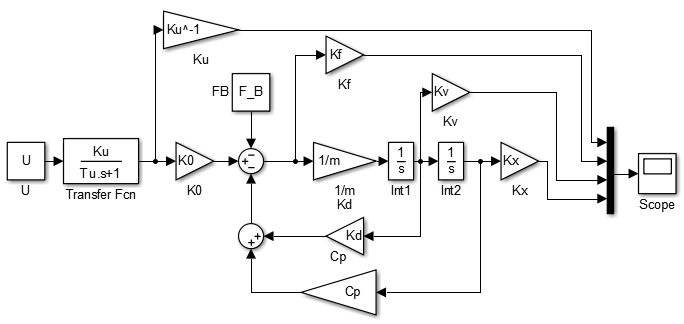
\includegraphics[scale=0.9]{images/model.png}
	\caption{Структурная схема пьезоэлектрического исполнительного устройства}
\end{figure}
\par 
Коэффициенты $K_u,\ K_V,\ K_X,\ K_F$ выбираются таким образом, чтобы обеспечить соответствие максимального значения измеряемого сигнала уровню 10В на выходе измерительного устройства.
\begin{equation}
	\left[
	\begin{matrix}
		K_u = 30\\
		K_V = 1\\
		K_X = 3307\\
		K_F = 0.0066\\
	\end{matrix}
	\right.
\end{equation}
\par 
Промоделируем систему. Полученные данные представлены на рисунке 2.
\newpage
\begin{figure}[h!]
	\begin{subfigure}{0.5\textwidth}
	\centering
		\begin{tikzpicture}
			\begin{axis}[
				xmin = 0, 
				xmax = 0.008,
				xlabel = {\Large{$t,c$}},
				ylabel = {\Large{$\hat{U_p}$}},
				width = 230,
				height = 200,
				grid = major,
			]
			\addplot[line width = 1, draw = blue] table [x=t, y=U]
				{data/U_1.txt};
			\end{axis}
		\end{tikzpicture}
    \end{subfigure}
    \begin{subfigure}{0.5\textwidth}
	\centering
		\begin{tikzpicture}
			\begin{axis}[
				xmin = 0, 
				xmax = 0.008,
				xlabel = {\Large{$t,c$}},
				ylabel = {\Large{$\hat{F}$}},
				width = 230,
				height = 200,
				grid = both,
			]
			\addplot[line width = 1, draw = blue] table [x=t, y=F]
				{data/F_1.txt};
			\end{axis}
		\end{tikzpicture}
    \end{subfigure}
    
    \vspace{0.5cm}

    \begin{subfigure}{0.5\textwidth}
	\centering
		\begin{tikzpicture}
			\begin{axis}[
				xmin = 0, 
				xmax = 0.008,
				xlabel = {\Large{$t,c$}},
				ylabel = {\Large{$\hat{V}$}},
				width = 230,
				height = 200,
				grid = both,
			]

			\addplot[line width = 1, draw = blue] table [x=t, y=V]
				{data/V_1.txt};
			\end{axis}
		\end{tikzpicture}
    \end{subfigure}
    \begin{subfigure}{0.5\textwidth}
	\centering
		\begin{tikzpicture}
			\begin{axis}[
				xmin = 0, 
				xmax = 0.008,
				xlabel = {\Large{$t,c$}},
				ylabel = {\Large{$\hat{X}$}},
				width = 230,
				height = 200,
				grid = both,
			]

			\addplot[line width = 1, draw = blue] table [x=t, y=X]
				{data/X_1.txt};
			\end{axis}
		\end{tikzpicture}
    \end{subfigure}
    \caption{Переходные процессы}
\end{figure}

\newpage
\section{Исследование влияния массы нагрузки $m$ на переходные процессы}
\par 
Диапазон изменения нагрузки: $\mp 50\%$ от заданного значения. Графики переходных процессов представлены на рисунке 3, а данные, полученные при моделировании - в таблице 2.
\begin{figure}[h!]
	\begin{subfigure}{0.5\textwidth}
	\centering
		\begin{tikzpicture}
			\begin{axis}[
				xmin = 0, 
				xmax = 0.001,			
				xlabel = {\Large{$t,c$}},
				ylabel = {\Large{$\hat{U},B$}},
				width = 220,
				height = 200,
				grid = both,
			]
			\addplot[line width = 1, draw = blue] table [x=t, y=m1]
				{data/U_2.txt};
			\end{axis}
		\end{tikzpicture}
    \end{subfigure}
    \begin{subfigure}{0.5\textwidth}
	\centering
		\begin{tikzpicture}
			\begin{axis}[
				xmin = 0, 
				xmax = 0.015,			
				xlabel = {\Large{$t,c$}},
				ylabel = {\Large{$\hat{F}$}},
				width = 220,
				height = 200,
				grid = both,
				%extra y ticks = {0.39, 0.78, 1.17, 1.56, 1.95},
				%ytick = {0, 4, 6},
				%scale only axis,
				enlarge y limits=0.05,
				legend style={nodes={scale=0.9, transform shape}}
			]

			\addplot[line width = 1, densely dashdotted, draw = blue] table [x=t, y=m1]
				{data/F_2.txt};
			\addplot[line width = 1, dashdotted, draw = red] table [x=t, y=m3]
				{data/F_2.txt};
			\addplot[line width = 1] table [x=t, y=m5] 
              	{data/F_2.txt};			
			\legend{
				$m = 0.0125\ \text{кг}$,
				$m = 0.025\ \text{кг}$,
				$m = 0.0375\ \text{кг}$	
				}
			\end{axis}
		\end{tikzpicture}
    \end{subfigure}
    
    \vspace{0.5cm}

    \begin{subfigure}{0.5\textwidth}
	\centering
		\begin{tikzpicture}
			\begin{axis}[
				xmin = 0, 
				xmax = 0.015,
				xlabel = {\Large{$t,c$}},
				ylabel = {\Large{$\hat{V}$}},
				width = 220,
				height = 200,
				grid = both,
				legend style={nodes={scale=0.9, transform shape}}
			]

			\addplot[line width = 1, densely dashdotted, draw = blue] table [x=t, y=m1]
				{data/V_2.txt};
			\addplot[line width = 1, dashdotted, draw = red] table [x=t, y=m3]
				{data/V_2.txt};
			\addplot[line width = 1] table [x=t, y=m5] 
              	{data/V_2.txt};			
			\legend{
				$m = 0.0125\ \text{кг}$,
				%$m = 0.01875\ \text{кг}$,
				$m = 0.025\ \text{кг}$,
				%$m = 0.03125\ \text{кг}$,
				$m = 0.0375\ \text{кг}$	
				}
			\end{axis}
		\end{tikzpicture}
    \end{subfigure}
    \begin{subfigure}{0.5\textwidth}
	\centering
		\begin{tikzpicture}
			\begin{axis}[
				xmin = 0, 
				xmax = 0.015,
				xlabel = {\Large{$t,c$}},
				ylabel = {\Large{$\hat{X}$}},
				width = 220,
				height = 200,
				grid = both,
				enlarge y limits = 0.05,
				legend style={nodes={scale=0.9, transform shape}},
				ytick = {0, 1, 3},
				extra y ticks = {2.015},
			]

			\addplot[line width = 1, densely dashdotted, draw = blue] table [x=t, y=m1]
				{data/X_2.txt};
			\addplot[line width = 1, dashdotted, draw = red] table [x=t, y=m3]
				{data/X_2.txt};
			\addplot[line width = 1] table [x=t, y=m5] 
              	{data/X_2.txt};			
			\legend{
				$m = 0.0125\ \text{кг}$,
				$m = 0.025\ \text{кг}$,
				$m = 0.0375\ \text{кг}$	
				}
			\end{axis}
		\end{tikzpicture}
    \end{subfigure}
    \caption{Переходные процессы при различных нагрузках $m$}
\end{figure}

\begin{table}[h!]
	\centering
	\begin{threeparttable}
	\caption{Результаты моделирования}\label{tab:perflogcross}
	\begin{tabular}{|c|c|c|c|}
		\hline
		$m,\text{кг}$ & $x_{уст}$ & $t_\text{п},c$ & $\sigma$\\
		\hline
		0.0125 & 2.015 & $2.114\cdot 10^{-3}$ & 0.55\\
		\hline
		0.025 & 2.015 & $1.78\cdot 10^{-3}$ & 0.67\\
		\hline
		0.375 & 2.015 & $7.37\cdot 10^{-3}$ & 0.73\\
		\hline
	\end{tabular}
	\end{threeparttable}
\end{table}

\newpage
\section{Исследование влияния $T_u$ на переходные процессы}
\par 
Переходные процессы при различных $T_u$ представлены на рисунке 4, а полученные данные в таблице 3.

\begin{figure}[h!]
	\begin{subfigure}{0.5\textwidth}
	\centering
		\begin{tikzpicture}
			\begin{axis}[
				xmin = 0, 
				xmax = 0.005,			
				xlabel = {\Large{$t,c$}},
				ylabel = {\Large{$\hat{U},B$}},
				width = 220,
				legend pos = south east,
				height = 200,
				grid = both,
			]
			\addplot[line width = 1, densely dashdotted, draw = blue] table [x=t, y=Tu2]
				{data/U_3.txt};
			\addplot[line width = 1, dashdotted, draw = red] table [x=t, y=Tu4]
				{data/U_3.txt};
			\addplot[line width = 1] table [x=t, y=Tu6] 
              	{data/U_3.txt};			
			\legend{
				$T_u = 0.1\ \text{мс}$,
				$T_u = 0.2\ \text{мс}$,
				$T_u = 0.3\ \text{мс}$	
				}
			\end{axis}
		\end{tikzpicture}
    \end{subfigure}
    \begin{subfigure}{0.5\textwidth}
	\centering
		\begin{tikzpicture}
			\begin{axis}[
				xmin = 0, 
				xmax = 0.005,			
				xlabel = {\Large{$t,c$}},
				ylabel = {\Large{$\hat{F}$}},
				width = 220,
				height = 200,
				grid = both,
				%extra y ticks = {0.39, 0.78, 1.17, 1.56, 1.95},
				%ytick = {0, 4, 6},
				%scale only axis,
				enlarge y limits=0.05,
				legend style={nodes={scale=0.9, transform shape}}
			]

			\addplot[line width = 1, densely dashdotted, draw = blue] table [x=t, y=Tu2]
				{data/F_3.txt};
			\addplot[line width = 1, dashdotted, draw = red] table [x=t, y=Tu4]
				{data/F_3.txt};
			\addplot[line width = 1] table [x=t, y=Tu6] 
              	{data/F_3.txt};			
			\legend{
				$T_u = 0.1\ \text{мс}$,
				$T_u = 0.2\ \text{мс}$,
				$T_u = 0.3\ \text{мс}$	
				}
			\end{axis}
		\end{tikzpicture}
    \end{subfigure}
    
    \vspace{0.5cm}

    \begin{subfigure}{0.5\textwidth}
	\centering
		\begin{tikzpicture}
			\begin{axis}[
				xmin = 0, 
				xmax = 0.005,
				xlabel = {\Large{$t,c$}},
				ylabel = {\Large{$\hat{V}$}},
				width = 220,
				height = 200,
				grid = both,
				legend style={nodes={scale=0.9, transform shape}}
			]

			\addplot[line width = 1, densely dashdotted, draw = blue] table [x=t, y=Tu2]
				{data/V_3.txt};
			\addplot[line width = 1, dashdotted, draw = red] table [x=t, y=Tu4]
				{data/V_3.txt};
			\addplot[line width = 1] table [x=t, y=Tu6] 
              	{data/V_3.txt};			
			\legend{
				$T_u = 0.1\ \text{мс}$,
				$T_u = 0.2\ \text{мс}$,
				$T_u = 0.3\ \text{мс}$	
				}
			\end{axis}
		\end{tikzpicture}
    \end{subfigure}
    \begin{subfigure}{0.5\textwidth}
	\centering
		\begin{tikzpicture}
			\begin{axis}[
				xmin = 0, 
				xmax = 0.005,
				xlabel = {\Large{$t,c$}},
				ylabel = {\Large{$\hat{X}$}},
				width = 220,
				height = 200,
				grid = both,
				legend pos = south east,
				enlarge y limits = 0.05,
				legend style={nodes={scale=0.9, transform shape}},
				ytick = {0, 1, 3},
				extra y ticks = {2.015},
			]

			\addplot[line width = 1, densely dashdotted, draw = blue] table [x=t, y=Tu2]
				{data/X_3.txt};
			\addplot[line width = 1, dashdotted, draw = red] table [x=t, y=Tu4]
				{data/X_3.txt};
			\addplot[line width = 1] table [x=t, y=Tu6] 
              	{data/X_3.txt};			
			\legend{
				$T_u = 0.1\ \text{мс}$,
				$T_u = 0.2\ \text{мс}$,
				$T_u = 0.3\ \text{мс}$	
				}
			\end{axis}
		\end{tikzpicture}
    \end{subfigure}
    \caption{Переходные процессы при различных $T_u$}
\end{figure}

\begin{table}[h!]
	\centering
	\begin{threeparttable}
	\caption{Результаты моделирования}\label{tab:perflogcross}
	\begin{tabular}{|c|c|c|c|}
		\hline
		$T_u,\text{мс}$ & $x_{уст}$ & $t_\text{п},c$ & $\sigma$\\
		\hline
		0.1 & 2.015 & $1.856\cdot 10^{-3}$ & 0.38\\
		\hline
		0.2 & 2.015 & $3.533\cdot 10^{-3}$ & 0.1\\
		\hline
		0.3 & 2.015 & $5.283\cdot 10^{-3}$ & 0.024\\
		\hline
	\end{tabular}
	\end{threeparttable}
\end{table}
\newpage
\par 
Рассчитаем корни характеристического уравнения системы, передаточная функция которой:
\begin{equation}
	W(s) = \displaystyle\frac{K_u(K_0U_{Pm}+F_B)}{(T_us+1)(ms^2+K_ds+Cp)}.
\end{equation}
\par 
Результаты расчётов представлены в таблице 4.
\begin{table}[h!]
	\centering
	\begin{threeparttable}
	\caption{Корни характеристического уравнения}\label{tab:perflogcross}
	\begin{tabular}{|c|c|c|c|}
		\hline
		$T_u,\text{мс}$ & $s_1$ & $s_2$ & $s_3$\\
		\hline
		0.1 & -10000 & -1600+11200j & -1600-11200j\\
		\hline
		0.2 & -5000 & -1600+11200j & -1600-11200j\\
		\hline
		0.3 & -3333 & -1600+11200j & -1600-11200j\\
		\hline
	\end{tabular}
	\end{threeparttable}
\end{table}

\newpage
\section{Исследование влияния возмущения $F_B$ при изменении $C_p$}
\par 
На рисунке 5 представлены графики переходных процессов при нулевом входном воздействии, внешнем возмущении и различных коэффициентах упругости.

\begin{figure}[h!]
    \begin{subfigure}{0.5\textwidth}
	\centering
		\begin{tikzpicture}
			\begin{axis}[
				xmin = 0, 
				xmax = 0.005,
				xlabel = {\Large{$t,c$}},
				ylabel = {\Large{$\hat{V}$}},
				width = 220,
				height = 200,
				grid = both,
				legend style={nodes={scale=0.9, transform shape}},
			]

			\addplot[line width = 1, densely dashdotted, draw = blue] table [x=t, y=Cp1]
				{data/V_4.txt};
			\addplot[line width = 1, dashdotted, draw = red] table [x=t, y=Cp2]
				{data/V_4.txt};		
			\legend{
				$C_p = 1.6\cdot 10^6 H/\text{м}$,
				$C_p = 6.4\cdot 10^6 H/\text{м}$,
				}
			\end{axis}
		\end{tikzpicture}
    \end{subfigure}
    \begin{subfigure}{0.5\textwidth}
	\centering
		\begin{tikzpicture}
			\begin{axis}[
				xmin = 0, 
				xmax = 0.005,
				xlabel = {\Large{$t,c$}},
				ylabel = {\Large{$\hat{X}$}},
				width = 220,
				height = 200,
				grid = both,
				legend pos = south east,
				enlarge y limits = 0.05,
				legend style={nodes={scale=0.9, transform shape}},
				ytick = {0},
				extra y ticks = {-0.00413359832758730,	-0.00103339951936819},
			]

			\addplot[line width = 1, densely dashdotted, draw = blue] table [x=t, y=Cp1]
				{data/X_4.txt};
			\addplot[line width = 1, dashdotted, draw = red] table [x=t, y=Cp2]
				{data/X_4.txt};		
			\legend{
				$C_p = 1.6\cdot 10^6 H/\text{м}$,
				$C_p = 6.4\cdot 10^6 H/\text{м}$,
				}
			\end{axis}
		\end{tikzpicture}
    \end{subfigure}
    \caption{Переходные процессы при различных $C_p$ и $F_B=2H$}
\end{figure}
\par 
Построим асимптотическую ЛАЧХ исполнительного устройства. Передаточная функция ИУ:
\begin{equation}
	W(s) = \displaystyle\frac{K_u(K_0U_{Pm}+F_B)}{(T_us+1)(ms^2+K_ds+Cp)}.
\end{equation}
\par
Найдём сопрягающие частоты и соответствующие им амплитуды:
\begin{equation}
	\begin{matrix}
		\omega_1 = \sqrt{\frac{m}{C_p}} = 11313.7\ c^{-1},\ L_1(\omega) = -34.76\text{дБ}, \\
		\omega_2 = \frac{1}{T_u} = 20000\ c^{-1},\ L_2(\omega) = -44.55\text{дБ}.\\
	\end{matrix}
\end{equation}
\par 
Составим асимптотическую ЛАЧХ ИУ, которая представлена на рисунке 6.
\newpage
\begin{figure}[h!]
	\centering
	\begin{tikzpicture}
		\begin{semilogxaxis}[
			height=9cm, width=16cm,
			xmin = 100,
			xmax = 10e+5,
			xlabel = {$\omega,c^{-1}$},
			ylabel = {$L(\omega),\text{дБ}$},
			grid = major,
			extra y ticks = {-34.76,-44.55},
			ytick = {-140, -120, -100, -80, -60},
			extra x ticks = {11313.7, 20000},
			xtick = {10e+1, 10e+2, 10e+4, 10e+5},
			extra x tick labels = {$\omega_1$,$\omega_2$},
		]
		\addplot[dashed,draw = red, line width = 1] table [x=w,y=L] {data/data.txt};
		\addplot[thick, blue, mark = *, mark options = {black}] coordinates {(100, -34.76) (11313.7,-34.76) (20000,-44.55) (10^6,-146.59)};
		\draw[dashed] (axis cs: 11313.7,-34.76) -- (axis cs: 11313.7,-160);
		\draw[dashed] (axis cs: 100, -44.55) -- (axis cs: 20000,-44.55) -- (axis cs: 20000,-160);
		\legend{$Model$, $Asymptotic$}
		\end{semilogxaxis}
	\end{tikzpicture}
	\caption{Промоделированная и асимптотическая ЛАЧХ ИУ}
\end{figure}

\newpage
\begin{center}	
	\section*{Вывод}
\end{center}
\par 
В лабораторной работе исследовалось исполнительное устройство на основе пьезодвигателя, его математическая модель, а также влияние изменения различных параметров($m$, $T_u$, $F_B$, $C_p$) на вид переходных процессов. 
\par 
При увеличении массы нагрузки увеличивается время переходного процесса, а также увеличением перерегулирования, что обусловлено снижением динамического усилия в пьезодвигателе.
\par 
При увеличении $T_u$ увеличивается время переходных процессов с уменьшением перерегулирования, что легко объяснить более плавным и медленным управлением выполняющим устройством.
\par 
При увеличении коэффициента упругости для нулевого входного воздействия и заданном $F_B$ уменьшается влияние внешних возмущений, а значит, ошибки. 
\par 
Сравнение смоделированной и асимптотической ЛАЧХ показало, что расчёты оказались верными, а графоаналитический метод - очень даже актуальным.
\end{document}
